\chapter{Software for emotion detection}
\label{ch:software}

During the systematic evaluation of the elements that compose the method proposed in this thesis, several software-based tests were performed. Additionally, all the data collection, e.g. HR estimations and facial actions, was carried out with custom made software. The previously mentioned automated facial analysis, responsible for collecting facial cues from videos, is an example. Each of these code components was incorporated in a software, which can be seen as a partial instantiation of the artifact produced as the outcome of this research. Figure \ref{fig:readmind-main-window} shows the software working on a video file. This chapter details each of these components and how they were unified in a single software that can be used to collect data for the remote estimation of the emotional states of a player interacting with games.

\begin{figure}[h!]
    \centering
    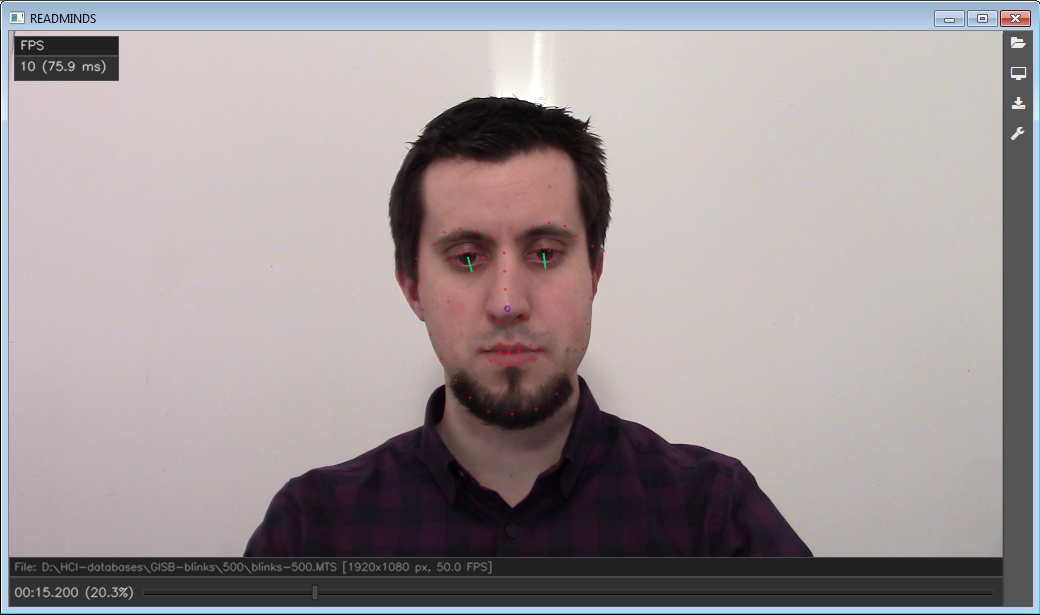
\includegraphics[width=\textwidth]{Content/figures/tool-main-window.png}
    \caption{Software developed as a partial instantiation of the proposed method working on a video file. Detected facial points and eye gaze information are superimposed on each frame of the video.}
    \label{fig:readmind-main-window}
\end{figure}

\section{Overall structure}

The software was mainly developed in C++ using the computer vision library OpenCV \parencite{opencv_library}. The overall structure of the software is illustrated in Figure \ref{fig:tool-overall-structure}. The system contains six main components, i.e. emotion model, emotion estimator, face detector, signal estimator, face analyzer, and report manager, which work in conjunction with two auxiliary components, i.e. video manager and UI. The two auxiliary components are not relevant to the scope of this thesis, however, they perform tasks related to reading video files, providing raw data to other components, i.e. frames of any loaded video, and allowing interactions with the operator, i.e. adjustment of parameters. The following sections explain in detail the main components of the software.

\begin{figure}
    \centering
    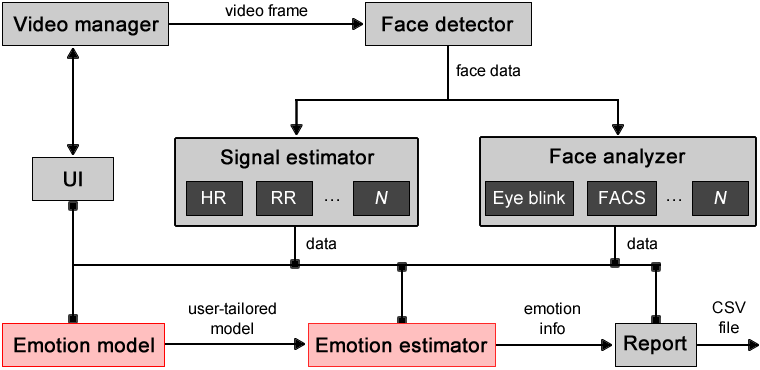
\includegraphics[width=0.8\textwidth]{Content/figures/tool-overall-structure.png}
    \caption{Overall structure of the software and its components.}
    \label{fig:tool-overall-structure}
\end{figure}

\subsection{Face detector}

The face detector component locates a human face in a given frame read from the input video being analyzed. It performs a face alignment procedure using one of the two available algorithms: Constrained Local Neural Fields (CLNF) \parencite{baltrusaitis2013constrained} and Ensemble of Regression Trees (ERT) \parencite{kazemi2014one}. The face alignment procedure is based on existing implementations of CLNF and ERT provided by OpenFace \parencite{baltruvsaitis2016openface} and dlib \footnote{http://dlib.​net} \parencite{dlib09}, respectively.

\begin{figure}
    \centering
    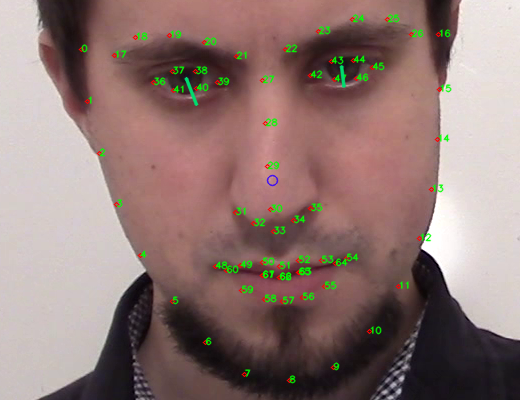
\includegraphics[width=0.6\textwidth]{Content/figures/tool-ui-face-detector.png}
    \caption{Visual representation of the 68 points detected as facial landmarks. Blue circle represents the average position (center of mass) of all detected facial landmarks.}
    \label{fig:tool-ui-face-detector}
\end{figure}

The output of the face detector is a vector containing 68 2D points, each one representing a facial landmark. Figure \ref{fig:tool-ui-face-detector} shows a visual representation of the mentioned vector and its points overlapped in a face.

\subsection{Face analyzer}

The face analyzer component uses a frame of the input video and the information related to facial landmarks provided by the face detector. The face analyzer uses that data to extract information regarding facial activity, e.g. eye area. The facial analyzer orchestrates a list of independent analyzers, each one responsible for extracting specific activity patterns, e.g. eye area. Figure \ref{fig:tool-ui-face-analyzer} shows the user interface regarding the data provided by the face analyzer.

\begin{figure}[h]
    \centering
    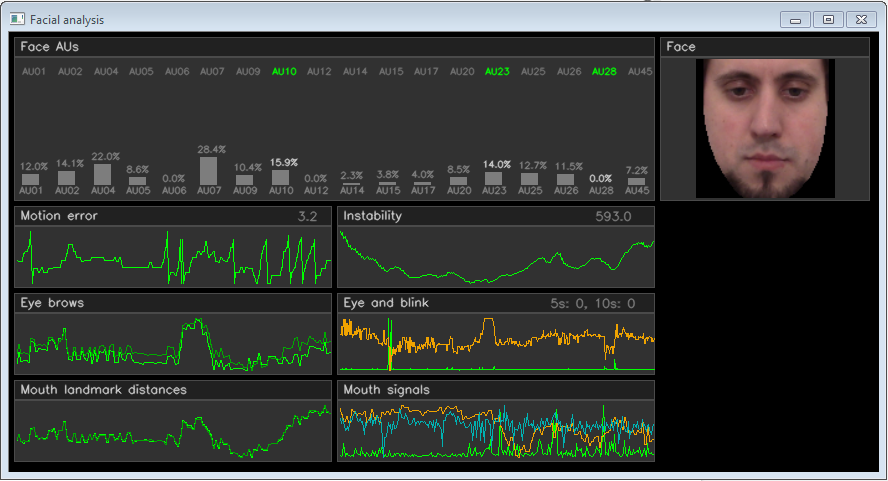
\includegraphics[width=0.8\textwidth]{Content/figures/tool-ui-face-analyzer.png}
    \caption{Visualization of data provided by the face analyzer. Available information: FACS AUs, detected face, motion and instability of the face, and variations of eye/mouth areas over time.}
    \label{fig:tool-ui-face-analyzer}
\end{figure}

Available analyzers extract information regarding eye (including eyebrow activity), mouth (lips/mouth activity), facial center of mass (mean position of all detected landmarks), distance among facial landmarks, face instability (including measurement of movement/rotation of the face), head movement, FACS facial action units (based on the implementation of \textcite{baltruvsaitis2015cross}), and eye gaze tracking (based on the implementation of \textcite{wood2015rendering}).

\subsection{Signal estimator}

The signal estimator component works similarly to the face analyzer, however, it uses input video frames and located facial landmarks to estimate physiological signals, e.g. HR. It contains different estimators, each one responsible for estimating a single signals. There are two signal estimators available, both estimate HR by using different techniques. These estimators use ICA-based rPPG techniques \parencite{poh2010non,poh2011advancements} implemented in Matlab.

\begin{figure}[h]
    \centering
    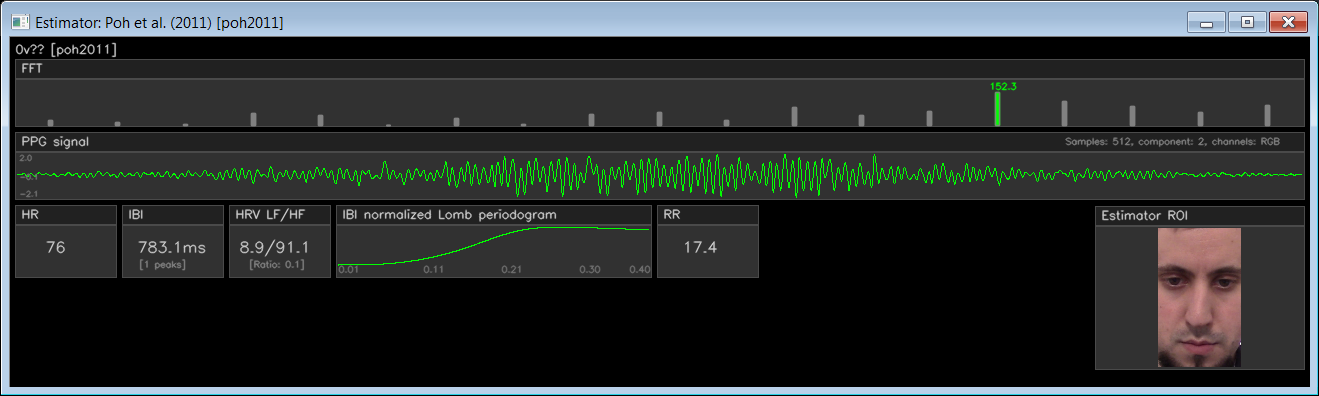
\includegraphics[width=0.8\textwidth]{Content/figures/tool-ui-signal-estimator.png}
    \caption{Visualization of data provided by the signal estimator. Available information: most prominent frequencies detected, photoplethysmographic signal, estimated HR, and the ROI used in the estimation.}
    \label{fig:tool-ui-signal-estimator}
\end{figure}

Figure \ref{fig:tool-ui-signal-estimator} shows the user interface regarding the data provided by the signal estimator. Available information provided by the signal estimator include the photoplethysmographic signal, estimated HR, and the ROI used in the estimation.

\subsection{Report manager}

The report component aggregates the information produced by other components, generating a CSV report file as output. The report files contain information regarding the video, e.g. time, as well as estimated signals and extracted facial activity. The file generated by the report manager is used to exchange information between the software and third-party systems, e.g. software for statistical analysis. The report file is also used by the two components related to emotion modeling and estimation, as explained in the next section.

\subsection{Emotion model and estimator}

Finally the emotion model and the emotion estimator components are responsible for training the user-tailored model and applying it, respectively. Both components were developed in R using the \texttt{caret} package for machine learning. The components work on the report file produced by the report manager.
